%% This is file `elsarticle-template-5-harv.tex',
%%
%% Copyright 2009 Elsevier Ltd
%%
%% This file is part of the 'Elsarticle Bundle'.
%% ---------------------------------------------
%%
%% It may be distributed under the conditions of the LaTeX Project Public
%% License, either version 1.2 of this license or (at your option) any
%% later version.  The latest version of this license is in
%%    http://www.latex-project.org/lppl.txt
%% and version 1.2 or later is part of all distributions of LaTeX
%% version 1999/12/01 or later.
%%
%% The list of all files belonging to the 'Elsarticle Bundle' is
%% given in the file `manifest.txt'.
%%
%% Template article for Elsevier's document class `elsarticle'
%% with harvard style bibliographic references
%%
%% $Id: elsarticle-template-5-harv.tex 159 2009-10-08 06:08:33Z rishi $
%% $URL: http://lenova.river-valley.com/svn/elsbst/trunk/elsarticle-template-5-harv.tex $
%%
\documentclass[preprint,authoryear,12pt]{elsarticle}

%% Use the option review to obtain double line spacing
%% \documentclass[authoryear,preprint,review,12pt]{elsarticle}

%% Use the options 1p,twocolumn; 3p; 3p,twocolumn; 5p; or 5p,twocolumn
%% for a journal layout:
%% \documentclass[final,authoryear,1p,times]{elsarticle}
%% \documentclass[final,authoryear,1p,times,twocolumn]{elsarticle}
%% \documentclass[final,authoryear,3p,times]{elsarticle}
%% \documentclass[final,authoryear,3p,times,twocolumn]{elsarticle}
%% \documentclass[final,authoryear,5p,times]{elsarticle}
%% \documentclass[final,authoryear,5p,times,twocolumn]{elsarticle}

%% if you use PostScript figures in your article
%% use the graphics package for simple commands
%% \usepackage{graphics}
%% or use the graphicx package for more complicated commands
%% \usepackage{graphicx}
%% or use the epsfig package if you prefer to use the old commands
%% \usepackage{epsfig}

%% The amssymb package provides various useful mathematical symbols
\usepackage{amssymb}
%% The amsthm package provides extended theorem environments
%% \usepackage{amsthm}
\usepackage{color}
\usepackage{siunitx}
\usepackage{array}

%% The lineno packages adds line numbers. Start line numbering with
%% \begin{linenumbers}, end it with \end{linenumbers}. Or switch it on
%% for the whole article with \linenumbers after \end{frontmatter}.
%% \usepackage{lineno}

%% natbib.sty is loaded by default. However, natbib options can be
%% provided with \biboptions{...} command. Following options are
%% valid:

%%   round  -  round parentheses are used (default)
%%   square -  square brackets are used   [option]
%%   curly  -  curly braces are used      {option}
%%   angle  -  angle brackets are used    <option>
%%   semicolon  -  multiple citations separated by semi-colon (default)
%%   colon  - same as semicolon, an earlier confusion
%%   comma  -  separated by comma
%%   authoryear - selects author-year citations (default)
%%   numbers-  selects numerical citations
%%   super  -  numerical citations as superscripts
%%   sort   -  sorts multiple citations according to order in ref. list
%%   sort&compress   -  like sort, but also compresses numerical citations
%%   compress - compresses without sorting
%%   longnamesfirst  -  makes first citation full author list
%%
%% \biboptions{longnamesfirst,comma}

% \biboptions{}

\journal{Biosystems Engineering}

\begin{document}

\begin{frontmatter}

%% Title, authors and addresses

%% use the tnoteref command within \title for footnotes;
%% use the tnotetext command for the associated footnote;
%% use the fnref command within \author or \address for footnotes;
%% use the fntext command for the associated footnote;
%% use the corref command within \author for corresponding author footnotes;
%% use the cortext command for the associated footnote;
%% use the ead command for the email address,
%% and the form \ead[url] for the home page:
%%
%% \title{Title\tnoteref{label1}}
%% \tnotetext[label1]{}
%% \author{Name\corref{cor1}\fnref{label2}}
%% \ead{email address}
%% \ead[url]{home page}
%% \fntext[label2]{}
%% \cortext[cor1]{}
%% \address{Address\fnref{label3}}
%% \fntext[label3]{}

% \title{An Autonomous Platform for Use in Kiwifruit Orchards}
\title{A Platform for Autonomous Navigation of Kiwifruit Orchards}

%% use optional labels to link authors explicitly to addresses:
%% \author[label1,label2]{<author name>}
%% \address[label1]{<address>}
%% \address[label2]{<address>}

% \author{Mark H. Jones, Jamie Bell, Matthew Seabright, Joshua Barnett, Alistair Scarfe, Bruce MacDonald, Mike Duke}

%% Group authors per affiliation:
\author[UoW]{Mark H. Jones\corref{mjemail}} 
\cortext[mjemail]{markj@waikato.ac.nz}

\author[UoA]{Jamie Bell\corref{jbemail}}
\cortext[jbemail]{jamie977@gmail.com}
\author[UoW]{Matthew Seabright}
\author[RPL]{Alistair Scarfe}
\author[UoW]{Mike Duke}
\author[UoA]{Bruce MacDonald}

\address[UoW]{School of Engineering, University of Waikato, Hamilton, New Zealand}
\address[UoA]{Faculty of Engineering, University of Auckland, Auckland, New Zealand}
\address[RPL]{Robotics Plus Ltd, Newnham Innovation Park, Tauranga, New Zealand}

\begin{abstract}
%% Text of abstract

    This will be written last.
    General tone of paper is:
    We present a vehicle designed specifically for autonomous control in kiwifruit orchards.
    Here are some other people who have made autonomous specific vehicles.
    Here is ours and this is how it fits in with those.
    We've gone with these sensors and this method of navigation and it has demonstrated itself to work in the orchard.
    We think that we could improve the thing by using this algorithm and increasing module space.
    Generally it is an improvement on the previous work of Scarfe.
\end{abstract}

\begin{keyword}
%% keywords here, in the form: keyword \sep keyword

%% MSC codes here, in the form: \MSC code \sep code
%% or \MSC[2008] code \sep code (2000 is the default)
    Agricultural robotics \sep outdoor navigation \sep
\end{keyword}

\end{frontmatter}

% \linenumbers

%% main text
\section{Introduction}
\label{sect:intro}
    Short-term labor requirements within New Zealand's kiwifruit industry peak twice a year corresponding with pollination and harvesting.
    The majority of employment during these peaks is filled by seasonal or casual workers \citep{Timmins2009}.
    As kiwifruit is the country's largest horticultural export by value \citep{StatisticsNewZealand2015}, automation in this industry may promote economic growth.
    % The New Zealand government aims to double exports from its primary industries between 2012 and 2025 and is actively investing in programmes to achieve this \citep{MinistryPrimaryIndustries2015}.

    Previous work on automated harvesting of kiwifruit has been demonstrated \citep{Scarfe2012,scarfe2009}.
    That work presents a mobile platform integrated with robotic arms that is capable of harvesting pergola type kiwifruit orchards.
    The platform presented in this paper is a second generation unit that increases modularity by separating the platform from the tasks it performs.
    This work discusses only the base platform, where details of modules for harvesting and pollination are published separately \citep{williams2017,Seabright2017}.

    Automation in kiwifruit harvesting and pollinating demands computer control, state-of-the-art manipulators, and convolutional neural networks.
    These systems are bulky and have specific geometric requirements dictated the environment and the tasks they perform.
    They share the requirements of transport to and from orchards, electrical power, and air pressure, but differ in they way they move when in the orchard.
    The pollinating module moves at a well-known velocity with minimum changes in angle, whereas the harvester advances a set distance between stationary harvest cycles.
    The duration of such harvesting cycles are determined by the number of fruit available during any particular cycle.
    As the harvester is designed to be autonomous, there must be communication between the platform and harvester to trigger forward movement between cycles.

    It has been stated that ``since the robot development already includes a high complexity, the application itself should be of comparably low complexity'' \citep{Ruckelshausen2009}.
    By separating development of the base platform from the task-specific modules, risk of over-complexity is reduced by way of separation.
    The platform presented here simply needs to transport task specific modules autonomously through kiwifruit orchards.

    The development of autonomous vehicles in agriculture is not new, but much of the literature relates to existing vehicles converted to driverless.
    This work details the development of a purpose-built platform for carrying robotic modules through an orchard environment.

    \begin{figure}[htb]
        \centering
        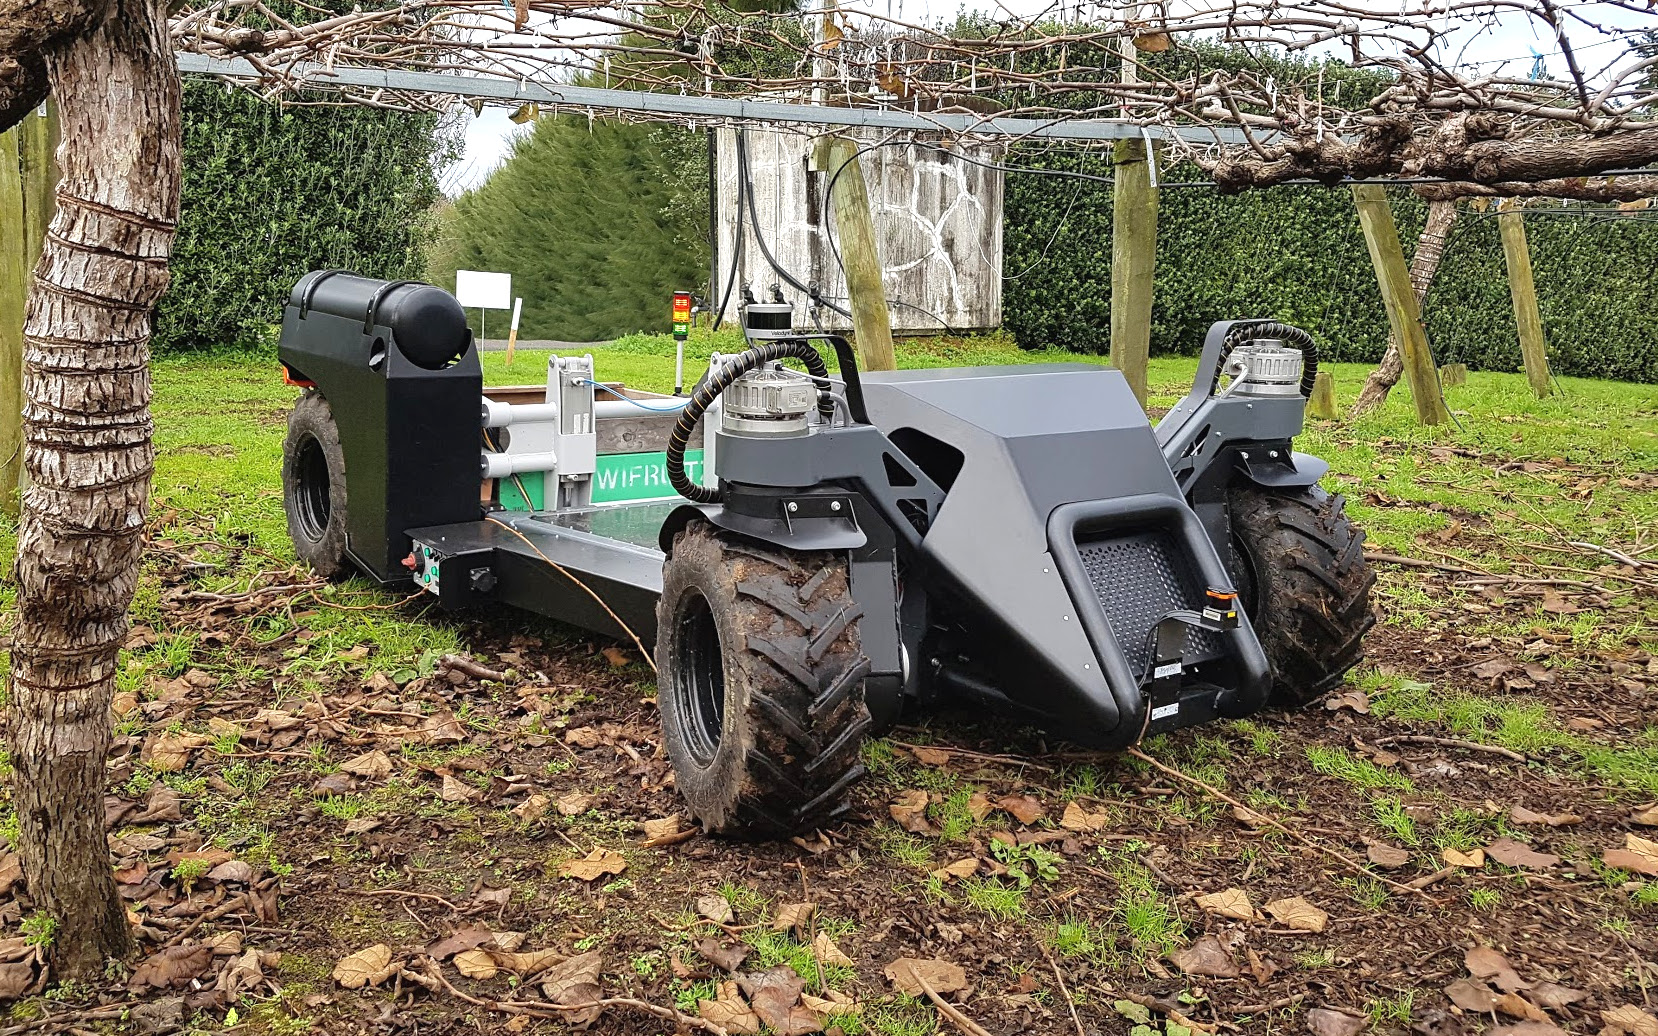
\includegraphics[width=\linewidth]{imgs/photos/suzy_general.jpg}
        \caption{
            The robot platform driving through a kiwifruit orchard.
        }
        \label{fig:suzy}
    \end{figure}

\section{Related Work}
\label{sect:review}

    \subsection{Purpose-built Autonomous Vehicles}

        The introduction of computers and digital camera technology during the 1980s sparked research into creating autonomous vehicles for agricultural use \cite{Li2009}.
        When publishing details of an autonomous vehicle in 1999, Tillett et~al.\@ cites difficulties dealing with variability in lighting and the environment as the reason no commercial ready vehicles were available at the time.
        Their vehicle combined wheel encoders, a compass, and accelerometers for odometry information, and featured a camera based row guidance system.
        It was capable of spraying individual plants whilst autonomously driving at \SI{2.5}{\kilo\meter\per\hour}.
        
        In 2002, two autonomous robots designed for weed mapping and control were published \citep{Pedersen2002,Astrand2002}.
        These platforms had relatively simple chassis and drive systems as they were both at a prototype stage.
        Both were Ackermann based and designed for field crops.
        The vehicle presented by \cite{Pedersen2002} was designed to follow pre-defined paths through row-crops, but the authors found that this was impractical without a dedicated row guidance sensor.
        They proposed a revision of their prototype that featured four wheel steering and drive system and integrating both GPS and a row guidance measurements.
        This work demonstrates a need to combine data from multiple sensor types, which becomes common.
        Mention at this time was made of utilising a Controller Area Network (CAN) to communicate with drive and steering modules on the revised unit due to it being a dominating standard in agricultural vehicles.
        \colorbox{yellow}{Did this next prototype ever get published?}
        
        \cite{Bak2004} present a relatively advanced robotic platform based on a four wheel steering geometry.
        The authors noted that the control strategy for the four independently controlled wheels was non-trivial.
        Like the platform presented earlier by Pederson et~al.\@, it combined a compass, gyroscope and GPS for odommetry.
        However, it also featured encoder feedback, a row detection sensor and a GPS unit utilising Real Time Kinematic (RTK) corrections from a base station.
        RTK-GPS is capable of providing positioning with accuracies of around \SI{2}{\centi\meter}.
        Their robot utilised a CAN bus for some aspects of system communication.

        In 2008, Klose et~al.\@ publish details of `Weedy', a autonomous weed control robot for field use.
        It used a very simple four wheel steering geometry.
        There are few details on the sensor selection apart from mention of the use of cameras and `acoustic distance sensors'.
        Presumably the selection of drive geometry on this robot is a cost/complexity optimisation.
        It too makes use of a CAN bus for communication between on-board modules.

        The following year, many the same authors appearing on the `Weedy' paper published details an autonomous robotic platform with four wheel steering named BoniRob \citep{Ruckelshausen2009}.
        BoniRob had the ability raise and lower itself and alter its wheel placement by actuating the arms to which the motors are attached to.
        Similar to the unit presented by Bak et~al.\@ it features a gyroscope and RTK-GPS for localisation.
        It introduces the use of both 2D and 3D laser-scanning (or lidar) for perception and row detection.
        A CAN bus is used to control the low level systems (such as the drive control) and ethernet connections for higher level communication.
        The authors created a simulated model of the platform using Gazebo in which they could test the many-degrees-of-freedom drive system.

        Of particular relevance to this work is that of Scarfe et~al.\@ on an autonomous kiwifruit picking robot \citep{scarfe2009, Scarfe2012}.
        That work involved the creation of a hydraulically driven platform with Ackermann steering to which four fruit harvesting arms were integrated.
        While its ability to navigate a kiwifruit orchard was not tested, it formed the foundation for the second-generation platform we present here.
        
        \cite{Blackmore2007} envisaged significant reductions in production costs by re-purposing parts already in use in the agricultural and automotive industry.
        While not a physical component, the CAN is one such technology borrowed from the automotive industry aiding developmental of low-level communications.
        Many of the platforms reviewed, especially the more recent ones, made use of this protocol for real-time communication.
        Platforms designed for open field crops appear to favor four-wheel steering over the more traditional Ackermann geometry.
        The use of simulation tools allowed the creators of BoniRob to develop and test their mobility system separate of the physical hardware.

        Common among these vehicles is the use of sensor fusion, whereby data from multiple sensors is merged and filtered.
        This provides a way to combine the advantages of multiple sensor types, and the benefit of redundancy  into a single computation space.
        With regards to the use of RTK-GPS in perception based guidance systems, Slaughter et~al.\@ points out the trade-off of requiring an ``unobstructed ``view'' of the sky from all parts of the field'' \citep{Slaughter2008}.
        Additionally, multi-path signal propagation caused by nearby foliage or the geometry of the land itself presents its own mode of failure \citep{Durrant-Whyte2005}.
        This requirement can not be satisfied under the canopy of a kiwifruit orchard which are usually surrounded by tall wind-breaking hedges.
        A separate feasibility analysis highlighted the use of RTK-GPS systems as a significant cost in yearly subscriptions alone \citep{Pedersen2006}.
        Torii suggests a combination of both RTK-GPS and machine vision systems to be the most promising system going forward based on reductions in costs and increases in performance of these systems \cite{Torii2000}.
        While \cite{Li2009} concludes that either GPS and machine vision, or GPS and lidar will be used together as a development trend.

    \subsection{Sensors for Row Based Navigation in Orchards}

        Sensors for orchard based row detection fall into two three categories; camera based, lidar based, or a combination of the two.
        The following section summarises a review of row detection efforts in orchards using these techniques.
        % Lidar come in two flavours: single-plane, and multi-plane.

        \cite{Subramanian2006} tested both camera based guidance and lidar (Sick LMS-200) based guidance systems in a citrus fruit orchard.
        Sensors were trialled separately on a tractor retrofitted with a fly-by-wire system.
        Their vehicle was able to navigate a small and simplified path using both machine vision and lidar based approaches at speeds of up to \SI{4.4}{\meter\per\second}.
        Lidar proved more accurate to the point at which the data rate became a limiting factor, after which image based approach became favourable.
        They suggest that combining the two systems would give more robust guidance as well as providing the ability to detect obstacles.
        No mention of the ability for the image based approach to cope with varying conditions is made.

        \cite{Barawid2007} demonstrate the use of data from a single-plane lidar (Sick LMS-219) being used to control a drive-by-wire tractor through an orchard.
        Their results show real-time processing of lidar data is sufficient to navigate an orchard at \SI{0.36}{\meter\per\second} (\SI{1.3}{\kilo\meter\per\hour}).

        \cite{Hansen2011} show the use of a single-plane lidar (Sick LMS-200) for vehicle localisation in an orchard.
        Also in 2011, two groups publish work on the generation of centre-lines from camera data of orchard rows.
        \cite{He2011} uses traditional machine vision, where \cite{Torres2011} makes use of neural network based image processing.
        Both methods generate valid paths, alghouth He et~al.\@ note that theirs may not be suitable when the envirnoment background becomes complex.

        The work of \cite{Scarfe2012}, combined traditional camera based image processing techniques with a single-plane lidar (Sick LMS-111).
        The image based approach failed to cope with variability in lighting conditions, however the lidar proved useful for detecting the trunks and posts of the row.

        \cite{Freitas2012} focus on the detection of people and bins in the rows of an apple orchard using lidar (Sick LMS-291), a low-cost inertial measurement unit, and wheel encoders.
        Their algorithm was capable of detecting each obstacle classe off-line from data captured in an apple orchard.

        \cite{Zhang2014} use a lidar (Hokuyo UTM-30LX) to generate maps of an apple orchard with the aid of artificial landmarks.
        They use an actuated single-plane lidar to generate multi-plane data for use in row and landmark sensing.
        Placing artificial land-marks in orchards is designed to reduce the effort required to create orchard maps for guidance systems.

        The following year, many of the same authors write about their autonomous vehicle \citep{Bergerman2015}.
        It describes a electric utility vehicle converted to fly-by-wire with the addition wheel encoders for odometry and a single-plane lidar (Sick LMS-111).
        While not able to detect obstacles in real-time, their previous work processing off-line data \citep{Freitas2012} has potential to be integrated with the addition of extra computing capability.

        Most recently, \cite{Sharifi2015} write about a method to generate a centre-line from an image an of an orchard rows.
        Like the work of \cite{He2011}, the technique offers a way to generate paths from a single camera image without resorting to neural networks.
        However, their future work focuses on increasing robustness to variations in lighting conditions, which indicates issues in this area.
        They state their system has use in being complementary to lidar based navigation.

        These works show that traditional image based processing for navigation fails when the scene becomes complex or the lighting varies.
        Combining cameras with neural network based processing increases the robustness to environmental complexities, such as light or clutter.
        The experiences of \cite{Scarfe2012} and similar indicate that Lidar outputs data which requires less post-processing to be robust.
        The use of lidar has seen two of the reported vehicles navigate autonomously through orchard enviroments.



\section{Platform Design}

    \subsection{Vehicle Configuration}
    \label{sect:mechanical}

        \begin{figure}[htb]
            \centering
            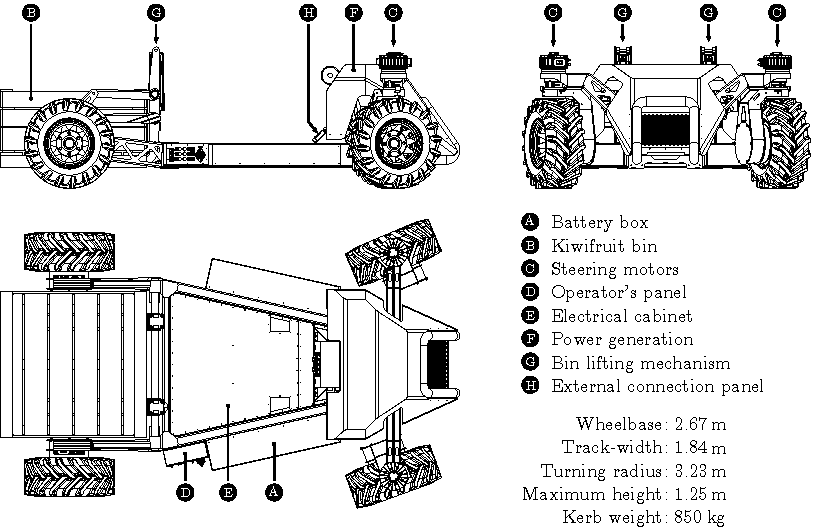
\includegraphics[width=\linewidth]{imgs/profile_views/AMMP-All-Labelled.pdf}
            \caption{Profile drawings of the robotic platform with kiwifruit bin.}
            \label{fig:AMMP}
        \end{figure}

        Modules designed to be carried by the platform require clearance from the canopy, in addition to to height they occupy themselves.
        A kiwifruit canopy ranges in height between \SI{1300}{\milli\meter} and \SI{1700}{\milli\meter}.
        To maximise space available to these modules the platform must be low-slung at the point of attachment.
        Figure \ref{fig:AMMP} illustrates the platform's design, with module area allocated between markers `F' and `E' in the side view (top left).
        The height of the chassis in this region is \SI{360}{\milli\meter} from the ground.

        Steering geometry is Ackermann based with independent motors on the front wheels for actuation.
        The ability to actuate the angles individually simplifies the mechanical geometry needed to coordinate steering, particularly at extreme steering angles.
        Steered wheels have the freedom to rotate \SI{340}{\degree}, limited by a mechanical stop.
        This range of steering angle allows the vehicle to place the centre of rotation between its rear wheels.
        At this angle, the turning circle is equal to approximately twice the length of the vehicle.
        Implementing four wheel steering would allow the centre of rotation to move to the centre of the vehicle, decreasing the turning circle to the total length of the vehicle.
        However, headlands in kiwifruit orchards are sized for tractors to turn between rows, tractors which use Ackerman steering geometries.
        The implementation of Ackermann geometry on the platform simplifies the mechanical design, removes the need to develop ``non-trivial'' control strategies, and increases the usable area.
        A differential drive, or skid steer, system was expected to cause ground damage to a level considered unacceptable to orchard owners.

        Bin lifting forks are fitted to the area between the rear wheels.
        This area is sized to accommodate a standard kiwifruit bin.
        The lifter is actuated by two vertically mounted pneumatic cylinders and is controlled by a standard pneumatic valve block.
        With this, the platform will have the ability to pick and place bins while operating in the orchard.

        Other than its tires, the platform has no suspension.
        It features a front pivoting axle that ensures that a minimum of three wheels are always in contact with the ground.
        Each wheel is mounted directly to a 40:1 fixed ratio planetary gearbox connected to a permanent magnet brushless AC motor.
        This specific gearbox-motor combination allows the platform to travel at a maximum speed of \SI{10}{\kilo\meter\per\hour}.
        The lack of suspension is not an issue when operating in orchards at this speed.
        In total, the drive system can continuously deliver \SI{25.6}{\kilo\watt} of power and \SI{3.3}{\kilo\newton\meter} of torque.
        Based on these specifications it is capable of accelerating from a stand-still to its maximum speed at an incline of \SI{20}{\degree} whilst carrying a \SI{600}{\kilo\gram} payload in \SI{2.0}{\second}.

        A power generation unit including a petrol engine, air compressor, and alternator is fitted at the front of the vehicle.
        The drive shafts of each are connected by a heavy-duty timing belt.
        The compressor and alternator are activated electronically by an embedded controller module.
        Fuel and compressed air tanks sit over the right-hand rear wheel, these can be seen in figure \ref{fig:suzy}.
        Battery modules attached to the sides of the chassis each house fifteen lithium-iron-phosphate batteries (thirty batteries in total).

        Unloaded, the machine has an estimated mass of \SI{850}{\kilo\gram}, including the power generation unit.
        It is capable of carrying a \SI{1000}{\kilo\gram} payload.
        The mass of a standard bin of kiwifruit can be as much as \SI{400}{\kilo\gram}, leaving \SI{600}{\kilo\gram} for modules.
        % With that load, the platform's maneuverability and ability to brake or accelerate was not noticeably affected.


\section{Navigation Sensors}
\label{sect:sensors}
    The choice of sensors incorporated into a platform determines which approaches are available for navigation and object detection.
    This section details the sensor selection specific for use in kiwifruit orchards.
%     Sensor selection was a critical early step in the development of the navigation system for the AMMP because it dictated the direction of subsequent research. Four approaches were used in the process of sensor selection:
%     \begin{enumerate}
%         \item Conducting a literature survey of sensors previously used in orchard navigation and similar applications.
%         \item Surveying the features, specifications and cost of sensors available to purchase in order to perform a cost-benefit analysis.
%         \item Purchasing some sensors, based on the cost-benefit analysis, collecting data from the sensors in kiwifruit orchards and analysing the data to ensure that the sensors perform according to some minimum criteria in the orchard environment.
%         \item Developing simple algorithms for the sensor data to demonstrate that the sensors can perform the functions that they have been purchased for.
%     \end{enumerate}

% \subsection{Sensor Literature Survey}
%     From the existing literature, it seems that the existing sensors that have been commonly used for orchard navigation systems are cameras, 2D lidar, GPS, inertial sensors and encoders for odometry. Some examples are summarised in Table \ref{table:1}.

%     \begin{table}[h!]
%     \caption{Examples of sensors used in previous orchard navigation research.}
%     \centering
%     \begin{tabular}{ | m{3.2cm} | m{3.2cm}| m{6.2cm} | } 
%     \hline
%     \textbf{Reference} & \textbf{Application} & \textbf{Sensors} \\
%     \hline
%     Subramanian et al., 2006 & Citrus grove navigation & Angled down 2D lidar and camera (640x480) separately; steering encoder \\ 
%     \hline
%     Barawid et al., 2007 & Autonomous tractor & Horizontal 2D lidar \\ 
%     \hline
%     Hansen et al., 2011 & Autonomous orchard vehicle & Horizontal 2D lidar, fibre optic gyroscope, odometry (encoders) \\ 
%     \hline
%     He et al., 2011 & Orchard row detection & Camera (640x480) \\
%     \hline
%     Torres- Sospedra and Nebot, 2011 & Orchard row detection & Camera (640x480) \\
%     \hline
%     Scarfe, 2012 & Kiwifruit harvesting robot & Horizontal 2D lidar, fluxgate compass \\
%     \hline
%     Freitas et al., 2012  & Orchard robot obstacle detection & Angled down 2D lidar, wheel and steering encoders, low cost IMU \\
%     \hline
%     Zhang et al., 2013  & Orchard robot row following & Rotated 2D lidar; lidar rotation, wheel and steering encoders \\
%     \hline
%     Bergerman et al., 2015 & Autonomous orchard vehicle & Horizontal 2D lidar, wheel and steering encoders \\
%     \hline
%     Bargoti et al., 2015 & Apple orchard localisation & Vertical 2D lidar, Global Positioning Inertial Navigation System \\
%     \hline
%     Jagbrant et al., 2015 & Almond orchard localisation & Vertical 2D lidar, Global Positioning Inertial Navigation System \\
%     \hline
%     Sharifi and Chen, 2015 & Orchard row detection & Camera \\
%     \hline
%     \end{tabular}
%     \label{table:1}
%     \end{table}

\subsection{Sensor Selection}

    As the drive motors have built-in wheel encoders, odometry data is already available on the platform.
    Encoders from powered wheels give false readings if wheel slip occurs, so these sensors cannot be used for odomentry alone.
    The data they provide can be used to assist with mapping, localisation, and provide velocity feedback.

    \begin{table}[htbp]
        \centering
        \footnotesize
        \begin{tabular}{ l l} 
            \textbf{Sensor Type}   &\textbf{Possible Issues} \\ \hline
            GPS                    & Prone to signal loss from surrounding foiliage\\  \hline
            IMU                    & Error accumulation and thermal drift\\ \hline
            Digital Compass        & Can be affected by nearby metal structures\\ \hline
            Encoders               & Error accumulation \\ \hline
            Lidar                  & Reduced visibility in fog and heavy rain \\ \hline
            Time of Flight Cameras & Reduced visibility in sunlight, fog and heavy rain \\ \hline
            Cameras                & Reduced visibility in fog or direct sunlight \\ \hline
            Thermal Cameras        & Reduced visibility in conditions of low thermal contrast\\ \hline
        \end{tabular}
        \label{table:sensor_comparison}
        \caption{Sensor types considered for inclusion on the platform.}
    \end{table}

    Other sensors considered for inclusion on the platform, and their associated issues, are outlined in table \ref{table:sensor_comparison}.
    Factors influencing which sensors were trialled were the benefits and issues of each sensor type, success during previously reported usage, and availability at a commercially viable price-point.
    Results of this work suggested that lidar, cameras, and time-of-flight cameras offered the most functionality for navigation and object detection.
    Because localisation is such a key functionality, GPS was also tested.

 %    The costs of different sensors for a single unit were collated by contacting various manufacturers and suppliers; these results were used to estimate cost ranges for each sensor type.
    % The benefits and issues for each sensor type were noted, based on previous experience and results.
    % All of this information is summarised in Table \ref{table:2}.

 %    This data seemed to indictate that the sensors that deliver the most functionality are lidar, cameras and time of flight cameras.
    % In addition, these three sensor types are a reasonable price, at the lower end of their cost range; especially for time of flight cameras, although these sensors have a serious issue with degredation in performance in sunlight.
    % Because localisation is such a key functionality, GPS also seemed like an important option to test.
    % From this data and since the AMMP has built-in encoders, it seemed to make sense to use encoders to assist with mapping, localisation and velocity feedback.
    

    % \begin{table}[htbp]
    %     \centering
    %     \footnotesize
    %     \begin{tabular}{ l l l l } 
    %         \textbf{Sensor Type} &\textbf{Navigation Applications} &\textbf{Issues} \\ \hline
    %         GPS                    & Localisation, pose and velocity measurement                              & Signal loss\\  \hline
    %         IMU                    & Acceleration and angular velocity measurement                            & Thermal drift, error accululation \\ \hline
    %         Digital Compass        & Heading measurement                                                      & \\ \hline
    %         Encoders               & Dead reckoning, velocity measurement                                     & Error accululation \\ \hline
    %         Lidar                  & Mapping, localisation, pose and velocity measurement, obstacle detection & Reduced functionality in fog and heavier rain \\ \hline
    %         Time of Flight Cameras & Mapping, localisation, pose and velocity measurement, obstacle detection & Reduced functionality in sunlight conditions, fog and heavier rain \\ \hline
    %         Cameras                & Mapping, localisation, pose and velocity measurement, obstacle detection & Reduced functionality when visibility is low \\ \hline
    %         Thermal Cameras        & Pedestrian detection                                                     & Reduced functionality in conditions of low thermal constrast\\ \hline
    %         Radar                  & Object detection                                                         & \\            
    %     \end{tabular}
    %     \label{table:sensor_comparison}
    %     \caption{A sample of the sensors considered and parameters used for sensor selection for the AMMP navigation system.}
    % \end{table}


 %    \begin{table}[h!]
 %        \centering
 %        \footnotesize
 %        \begin{tabular}{ l l l l } 
 %            % \scriptsize \textbf{Sensor Type} & \scriptsize \textbf{Manufacturers Considered} &\scriptsize \textbf{Cost Range (USD)} &\scriptsize \textbf{Navigation Applications} &\scriptsize \textbf{Issues} \\ \hline
 %            % \scriptsize GPS & \scriptsize Ublox, Garmin, Omnistar & \scriptsize 50- 4000 per annum & \scriptsize Localisation, pose and velocity measurement &\scriptsize Signal loss under the kiwifruit canopy \\  \hline
 %            % \scriptsize IMU & \scriptsize InvenSense, Analog Devices & \scriptsize 50- 3000 & \scriptsize Acceleration and angular velocity measurement & \scriptsize Thermal drift, accumulated errors \\ \hline
 %            % \scriptsize Digital Compass & \scriptsize Honeywell, KVH & \scriptsize 50-500 & \scriptsize Heading measurement & \scriptsize \\ \hline
 %            % \scriptsize Encoders & \scriptsize CUI & \scriptsize 30-50 & \scriptsize Dead reckoning, velocity measurement & \scriptsize Accumulated errors \\ \hline
 %            % \scriptsize 2D Lidar & \scriptsize Hokuyo, SICK & \scriptsize 2000-10000 & \scriptsize Mapping, localisation, pose and velocity measurement, obstacle detection & \scriptsize Tend to not work well in fog and heavier rain \\ \hline
 %            % \scriptsize 3D Lidar & \scriptsize Velodyne, Quanergy, Neptec & \scriptsize 4000-90000 & \scriptsize Mapping, localisation, pose and velocity measurement, obstacle detection & \scriptsize Tend to not work well in fog and heavier rain \\ \hline
 %            % \scriptsize Time of Flight Cameras & \scriptsize Intel, Basler, Fotonic, Odos Imaging & \scriptsize 100-9000 & \scriptsize Mapping, localisation, pose and velocity measurement, obstacle detection & \scriptsize Tend to not work well in sunlight conditions, fog and heavier rain \\ \hline
 %            % \scriptsize Cameras & \scriptsize FLIR, Basler & \scriptsize 500-1500 & \scriptsize Mapping, localisation, pose and velocity measurement, obstacle detection & \scriptsize Tend to not work well when visibility is low \\ \hline
 %            % \scriptsize Thermal Cameras & \scriptsize FLIR, Optris & \scriptsize 3000-14000 & \scriptsize Pedestrian detection & \scriptsize In hot conditions, this sensor becomes less useful for pedestrian detection \\ \hline
 %            % \scriptsize Radar & \scriptsize Delphi & \scriptsize 3000-5000 & \scriptsize Object detection & \scriptsize \\
 %            % \hline
 %            \textbf{Sensor Type} & \textbf{Manufacturers Considered} &\textbf{Cost ($$USD)}\\ \hline
 %            GPS & Ublox, Garmin, Omnistar & 50-4000 per annum\\  \hline
 %            IMU & InvenSense, Analog Devices & 50-3000\\ \hline
 %            Digital Compass & Honeywell, KVH & 50-500\\ \hline
 %            Encoders & CUI & 30-50\\ \hline
 %            2D Lidar & Hokuyo, SICK & 2000-10000\\ \hline
 %            3D Lidar & Velodyne, Quanergy, Neptec & 4000-90000\\ \hline
 %            Time of Flight & Intel, Basler, Fotonic, Odos Imaging & 100-9000 \\ \hline
 %            Cameras & FLIR, Basler & 500-1500 \\ \hline
 %            Thermal Cameras & FLIR, Optris & 3000-14000 \\ \hline
 %            Radar & Delphi & 3000-5000 \\
 %        \end{tabular}
 %        \label{table:2}
 %        \caption{A sample of the sensors considered and parameters used for sensor selection for the AMMP navigation system.}
 %    \end{table}

\subsection{Data Collection and Inspection}
    The sensors that seemed important to test, based on both the literature survey and the cost-benefit analysis were lidar, cameras and GPS.
	In addition, time of flight cameras were considered, because they seemed to be a compelling option based on the cost-benefit analysis; especially if some of the less expensive models were found to work well in sunlight.
	It was also decided that encoders would be tested in favour of using an IMU because the encoders were built into the AMMP motors.
	Some data was collected from each sensor in order to decide which sensors to prototype algorithms for.

    \subsubsection{GPS Data Collection}
        Two GPS modules were tested.
    	Both were connected via serial to a Beaglebone Black single board  computer.
    	The GPS set-ups tested were:
        \begin{itemize}
          \item Ublox Neo-M8N module, selected for its superior navigation sensitivity of -167 dBm and internal Low Noise Amplifier (LNA), additional 20 dB gain/ 0.8 dB noise LNA and active circuitry for the 25mm square ceramic patch antenna.
          \item OmniSTAR 5120VBS module, with AX0 series antenna, with 34 dB gain/ 1.4 dB noise LNA.
    	The AX0 series antenna claims high multipath rejection.
        \end{itemize}
        The procedure used for data collection was:
        \begin{enumerate}
            \item A route through a kiwifruit orchard was planned and plotted on a satellite map. The route was designed to include long stretches underneath the canopy and some areas with a good view of the sky.
            \item The distance between post centres along the planned route was measured using a tape measure.
            \item The GPS data collection setups were turned on at the starting point of the planned route and were left to initialise for 30 minutes.
            \item The data collection unit was carried along the planned route, stopping at each pole. At each pole, the data collection unit was placed near to the pole in an orientation that was repeated for every pole along the route.
            \item Step 4 was repeated until the entire route had been traversed and every pole along the way had been (approximately) mapped by the data collection unit.
        \end{enumerate}

        It was noticed during testing that the signal quality lights on both GPS setups were regularly indicating loss of GPS fix.
    	Although the entire data collection procedure was performed, many of the results, such as the measurement of spacing between trees and performance, are far less significant than the regular loss of the GPS fix.

        The orchard used for the data collection was Bateman’s at 48 Newnham Road, Whakamarama, New Zealand.
    	A path followed and the corresponding GPS data collected from the different setups is shown in Figure \ref{fig:gpsResults}.
    	Note that the path followed was traversed twice- once going out and once returning.
    	The data was collected at a slow walking speed- the entire path of approximately 500 metres took in the order of 15 minutes to complete, including stops about every 5.5 metres within the orchard.
    	Multiple sets of data were collected but Figure \ref{fig:gpsResults} is indicative of the results.

        \begin{figure}[htb]
            \centering
            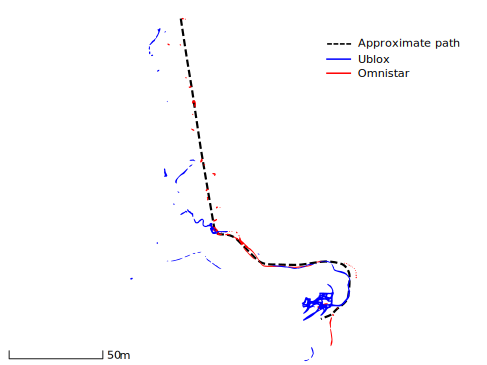
\includegraphics{imgs/gps_path/gps_path.pdf}
            \caption{
                Aerial view of a path through a kiwifruit orchard and the associated GPS data.
            }
            \label{fig:gpsResults}
        \end{figure}

        The Omnistar GPS setup appears to track the approximate path well but the data is sparse and there appears to be regular loss of signal in the orchard.
    	The Ublox GPS setup collected more data than the Omnistar setup but was much less accurate.
    	The conclusions of this work are that high quality GPS equipment may be useful to provide sanity checks of the approximate location in the orchard.
    	However, it was decided that GPS could not be relied on to provide localisation and other feedback, under the kiwifruit canopy.

    \subsubsection{Time of Flight Cameras}
        Two models of Time of Flight cameras were tested.
    	The first was the Basler TOF640-20GM-850NM.
    	This sensor provides depth and return signal data at a resolution of 640 pixels wide by 480 pixels high.
    	It was thought that this sensor migt work well in sunlight because it had previously been successfully used to collect data from the underside of the kiwifruit canopy in different lighting conditions, with minimal occurences of the data being washed out.
    	However, it was found that on bright sunny days and in overcast conditions, there was large amounts of data loss, which was deemed unacceptable for important navigation functions such as obstacle detection.

        The second time of flight sensor tested was an Intel RealSense R200.
    	The appealing characteristics of this sensor were its low cost and it was advertised as being able to work outdoors.
    	However, in overcast and sunny conditions, there was complete loss of range data.

    \subsubsection{Lidar Data Collection}
        Data was collected from two 2D lidar sensors; these were a Hokuyo UTM-30LX and a SICK LMS111.
    	Data was also collected from a 3D lidar sensor, which was a Velodyne VLP-16.
    	The data was collected by driving along rows in kiwifruit orchards with the sensors horizontal and at a height of 0.8 m, which was approximately midway between the ground and the canopy.

        The Hokuyo UTM-30LX exhibited some spurious unexplained measurements.
    	The cause of these erroneous measurements was not determined.

        \begin{figure}[htb]
            \centering
            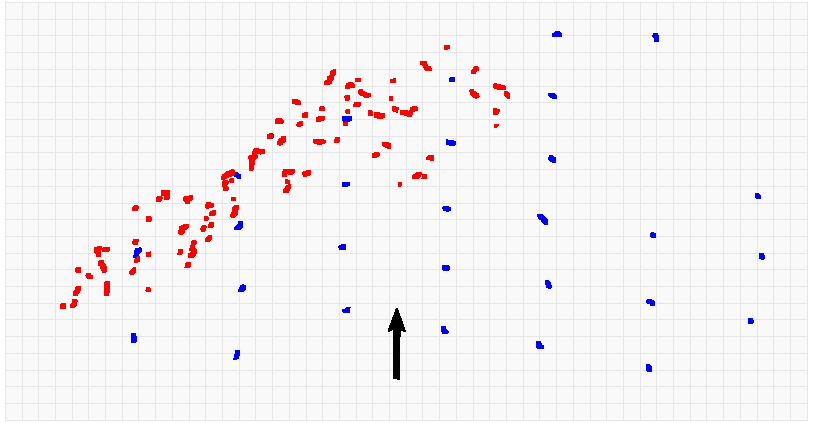
\includegraphics[width=\linewidth]{imgs/canopy_data/canopy_data.pdf}
            \caption{
                Captured lidar data showing the points reflected by the canopy (indicated by red markers) and points from tree trunks and posts (green markers).
                The arrow indicates the position and heading of the platform.
            }
            \label{fig:canopyDataCloud}
        \end{figure}

        It was thought that the lidar sensors would measure the position of structure defining features in the orchard, such as post, trunks and hedges.
    	Detecting such features would then allow the boundaries of the row to be found for row following or these features could be mapped and used for localisation.
    	However, both 2D lidar sensors produced clouds of unstructured data amongst the structured features, as shown in Figure \ref{fig:canopyDataCloud}.
    	This was caused by the lidar plane intercepting the canopy on convex slopes and, similarly intercepting the ground on concave slopes (Figure \ref{fig:concaveSlope}) at short ranges.

        \begin{figure}[htb]
            \centering
            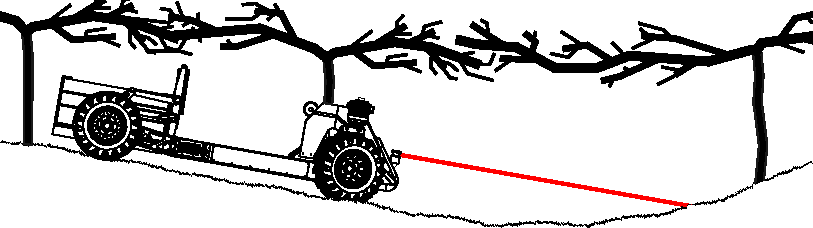
\includegraphics[width=\linewidth]{imgs/concave_slope/concave_slope_v4.pdf}
            \caption{
                On a concave slope the lidar scan plane may reflect off the ground instead of tree trunks and posts.
            }
            \label{fig:concaveSlope}
        \end{figure}

        Data was also collected from the 3D lidar sensor.
    	The 3D lidar sensor had 16 layers of data vertically.
    	As a result on concave slopes, some of the angled up planes had a longer viewing range facing forwards and on convex slopes some of the angled down planes had a longer viewing range facing forwards.

        From these results it seemed that the 2D lidar may be a useful sensor at a relatively short range to use for an independent channel of processing for redundancy and increased reliability.
    	However, it was decided to use 3D lidar as a primary navigation sensor because of its ability to be used at longer ranges on undulating ground in kiwifruit orchards.

    \subsubsection{Camera Data Collection}
        Data was collected from Logitech C920, Basler Dart daA1600-60uc and Flir CM3-U3-13S2C-CS cameras.
    	Data collection was performed at various times of the day and night, in different weather conditions and different orchards.
    	The data was collected on autonomous and manually driven platforms at a height of approximately 0.8 m from the ground and at speeds of up to 3 ms-1.
    	

        It was noticed that the Logitech C920 cameras produced significant motion blur.
    	In addition, these cameras did not provide a hardware trigger interface, which would be important if the cameras were used for stereovision.
    	No image quality issues were noticed with the Basler and Flir sensors; however, the Basler camera was favoured for its later model image sensor.

        In terms of sensor selection, the camera images seemed acceptable for performing object detection and classification.
    	This was checked by processing the data using readily accessible algorithms.

\subsection{Sensor Demonstration by Prototype Algorithm}
    The 3D lidar and cameras seemed to be the best of the sensors considered for use as the main sensors for the navigation system.
	The overall project goals for the navigation system fall into the following categories:
    \begin{itemize}
    \item Object detection and classification.
    \item Mapping and localisation.
    \item Driving through the rows of orchards.
    \end{itemize}
    In order to validate that the 3D lidar and camera could perform these functions, prototype navigation algorithms were created using these sensors.

\subsubsection{Object detection and classification}
    Object detection and classification was firstly prototyped fully on the camera data.
	It was decided to use a Convolutional Neural Network (CNN) for this purpose, because of the existing success of using CNNs for various image processing tasks \citep{LeCun2015}.
	The CNN architecture chosen was FCN-8s \citep{long2015}, which is a neural network made up of convolutional layers without fully connected layers, as opposed to having convolutional layers at the input and fully connected layers at the output.
	FCN-8s performs semantic segmentation, which is the per pixel labelling of images.
    In order to train the FCN-8s network, the camera image dataset, which was created in order assess the cameras for sensor selection, was reused and hand labelled.
	The hand labelling consisted of drawing outlines of objects of interest in an image, filling those outlines with colours that were defined to correspond to the given object, extracting the drawn pixels out onto a blank image and converting the result to a palleted indexed format.
	An example of an original image and a corresponding label image is shown in Figure \ref{fig:segImgLabelPair}.

    \begin{figure}[htb]
        \centering
        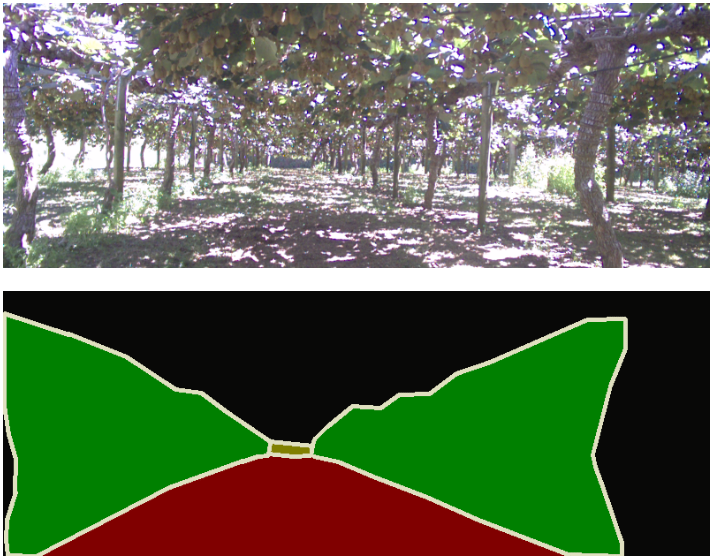
\includegraphics[width=\linewidth]{imgs/photos/segImgLabelPair.png}
        \caption{
            An input image (top) and labelled output (bottom) for semantic segmentation.
        }
        \label{fig:segImgLabelPair}
    \end{figure}

    Some experimentation was performed with labelling individual trees and posts in the kiwifruit orchard.
	However, what seemed to work best was to label the entire treeline, consisting of trees and posts as a single class.
	The list of objects that were labelled during algorithm prototyping were:
    \begin{itemize}
    \item The traversable space, which was defined as the ground in the image that the AMMP could drive a direct path to without collision.
    \item Treelines.
    \item The end of the row.
    \end{itemize}

    The labelled data was used to train an FCN-8s network.
	An example of the output from the trained network is shown in Figure \ref{fig:semSegRowResults}.

    \begin{figure}[htb]
        \centering
        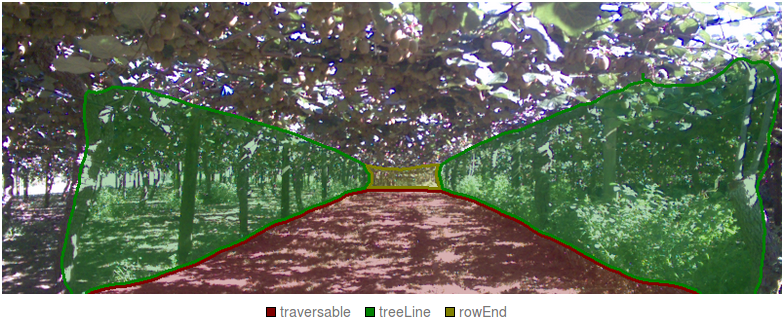
\includegraphics[width=\linewidth]{imgs/photos/semSegRowResults.png}
        \caption{
            An example result from the FCN-8s network, segmenting a kiwifruit orchard row.
        }
        \label{fig:semSegRowResults}
    \end{figure}

\subsubsection{Mapping and Localisation}
    In order to test the use of 3D lidar for mapping and localisation, an existing Simultaneous Localisation and Mapping (SLAM) package was used.
	The package used Gmapping \citep{Grisetti2007}, implemented as a ROS package \citep{Gerkey}.
	The required input for Gmapping was odometry data, which was provided by the wheel encoders, and a single plane of lidar data.
	The 3D lidar provides 16 planes of lidar data so a conversion had to be performed in order to produce a single plane of lidar data for Gmapping.
	The most simple approach of extracting a single plane out of the 16 planes from the 3D lidar sensor was not used because it was thought that this would produce the clouds of unstructured data, which was observed with the 2D lidar sensors.
	Instead, the approach initially used was:
    \begin{enumerate}
    \item The 4 lidar planes that were closest to horizontal were extracted.
	These planes were selected because they were the planes that generally detected the least amount of ground and canopy.
    \item For each angle of the lidar data, the difference in the range measurement between consecutive layers in the 4 lidar planes was calculated.
	
    \item If all of the differences between range measurements from step 2 at a given angle were less than a set threshold, the minimum of the ranges at that angle was extracted.
    \item Each extracted minimum range was used to populate a single plane of lidar data at the angle that the range was originally measured at.
    \end{enumerate}

    \begin{figure}[htb]
        \centering
        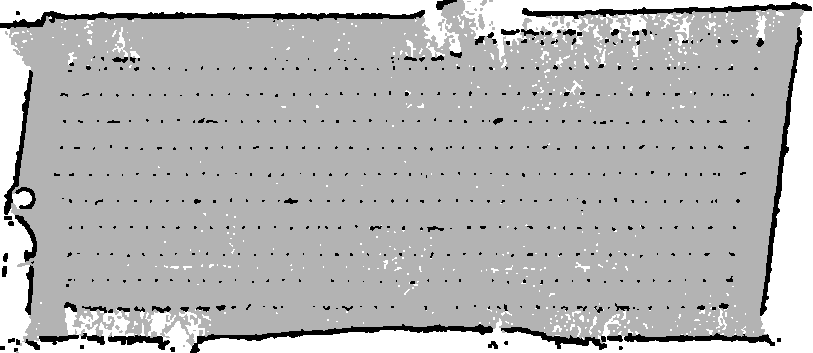
\includegraphics{imgs/gmapmap/gmapmap.pdf}
        \caption{
            A map of a kiwifruit orchard, created using GMapping, odometry data from encoders and a 3D lidar.
        }
        \label{fig:gmapmap}
    \end{figure}

    The output of these steps was a single plane of lidar data with reduced amounts of data from the canopy and ground at longer ranges.
	This data and the encoder data were used as the inputs for Gmapping.
	By driving along four rows of a kiwifruit block, the map in Figure \ref{fig:gmapmap}.

    \begin{figure}[htb]
        \centering
        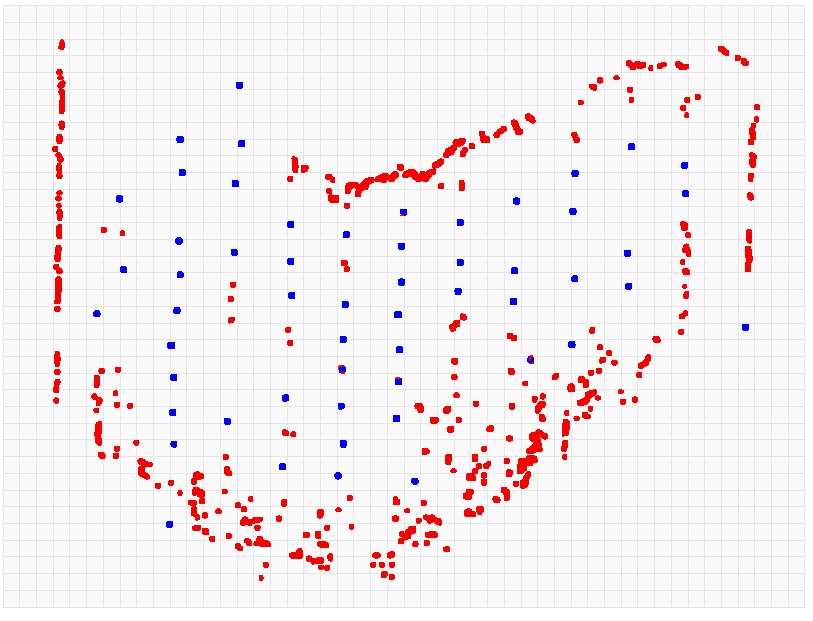
\includegraphics[width=\linewidth]{imgs/single_plane_extraction/single_plane_extraction.pdf}
        \caption{
            A single plane of the 3D lidar data. Points used for further processing are drawn in black and rejected points in red.
        }
        \label{fig:singlePlaneExtraction}
    \end{figure}

% \subsubsection{Orchard Driving Testing}
%     A 3D lidar navigation algorithm was developed and tested on smaller robot platforms, as described by Bell et al. \citep{Bell2016}. The key part of this algorithm was the calculation of the angular offset of the robot’s coordinate system from the row centreline. This algorithm attempted to extract the posts and trees from the lidar data and then find the angle between posts and trunks in the same treeline. The key steps of the algorithm were:
%     \begin{enumerate}
%     \item Clusters of close consecutive points were found in each plane of the 3D lidar data using the method described by Scarfe [24]⁠. 
%     \item Clusters with a length greater than a threshold were deemed to be unlikely to be row defining features, such as posts or trunks; as a result, these clusters were removed. 
%     \item Any clusters within a set distance of a set number of other clusters were also removed because these clusters could be a part of the clouds of data, which are returned from non structure defining features such as the kiwifruit canopy or the ground. An example result after this step for a single plane of the 3D lidar data is shown in Figure \ref{fig:singlePlaneExtraction}.
%     \item The clusters from multiple planes were grouped based on a threshold distance between clusters. 
%     \item The heights of the resulting groups from step 4 were compared to a threshold to determine which were posts and trees. An example result after this step for a single frame of 3D lidar data is shown in Figure \ref{fig:lastLidarFrame}.
%     \item Using the data from feature extraction, each cluster’s nearest neighbour was found. This step was taken because most posts and trunks are closer to other posts or trunks in the same tree-line than to an adjacent tree-line. This suggests that the angle between nearest neighbours should also be the angle of the tree-line. 
%     \item Nearest neighbours that were further apart than the row width were rejected to eliminate the possibility of using neighbours that were not in the same tree-line. 
%     \item The angles between the resulting nearest neighbours were calculated. 
%     \item The mode of the calculated angles was taken to be the current estimate of the angular offset of the robot from the row centreline. 
%     \end{enumerate}

%     Once the angular offset was found, the linear offset of the robot’s coordinate system origin from the row centreline was calculated. The steps used were:
%     \begin{enumerate}
%     \item The clusters belonging to the current row were found using the angular offset and the maximum row width for the orchard.
%     \item Lines were fitted to the treelines on the left and right sides of the row.
%     \item The row centreline was found as the average line from the left and right treelines.
%     \item The displacement of the robot centre from the row centreline was calculated.
%     \end{enumerate}

%     Row following was performed by calculating the steering angle from the sum of the proportional control signals for the linear and angular offsets. Row end detection was performed by detecting a volume of free space above the 3D lidar sensor. Row end driving was performed by driving a sequence of set curvature movements, while performing obstacle avoidance.

%     The autonomous driving algorithm described here has been used to drive 20 km autonomously on three different robot platforms, including the AMMP, in two different real kiwifruit orchards. This driving was performed using just lidar and encoder data. 
    
%     \begin{figure}[htb]
%         \centering
%         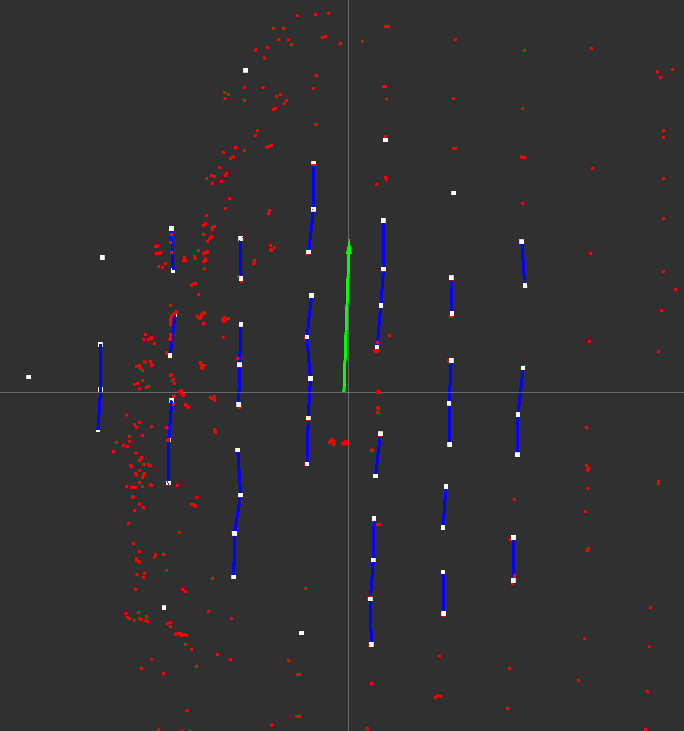
\includegraphics[width=\linewidth]{imgs/photos/lastLidarFrame.png}
%         \caption{
%             A single plane of 3D laser scanner data (red) with the points found by feature extraction highlighted in white, nearest neighbours indicated with blue and the detected row centreline (green arrow).
%         }
%         \label{fig:lastLidarFrame}
%     \end{figure}

\subsection{Sensor Selection Conclusions}
    The results from prototyping algorithms indicate that the 3D lidar and encoder sensors may be feasible selections for performing mapping, localisation and autonomous driving in kiwifruit orchards.
	Object detection using cameras in kiwifruit orchards also seems possible.
	Given these results with prototyping algorithms for the navigation system, it was decided to procede with using cameras, 3D lidar and encoders as the primary sensors for the navigation system.
	  









\section{System Architecture}
\label{sect:hardware}

    \newcommand{\rpm}{\raisebox{.2ex}{$\scriptstyle\pm$}}
    
    \begin{figure}[htb]
        \centering
        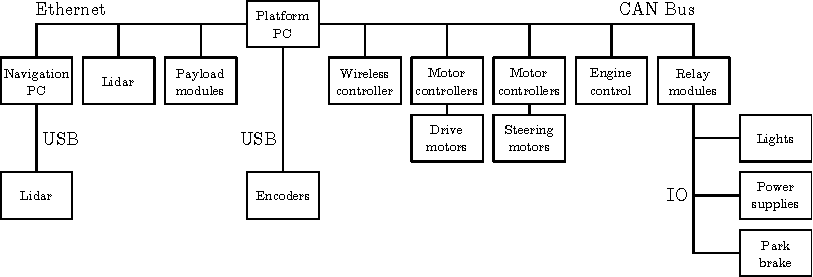
\includegraphics[width=\linewidth]{imgs/system_diagram/diagram_v3.pdf}
        \caption{Hardware level system diagram showing the types of interfaces and relative relations on the platform.}
        \label{fig:system_diagram}
    \end{figure}
    Sub-systems on the platform, including the drive system, are connected to the system PC via a CAN bus, as shown in figure \ref{fig:system_diagram}.
    The CANopen protocol has been implemented which offers message type prioritisation and a standardised way of sharing process data.
    Messages on the bus during operation are restricted to commands, syncronisation messages, and status updates.
    Relay modules connected to the bus allow the system to control the power to its on-board power supplies, motor controllers, park brakes, and lights.
    They also monitor the timing of synchronisation messages transmitted by the system PC and will enter an error state if the timing falls outside set limits.
    These messages must be transmitted every \SI{20}{\milli\second}, with a maximum allowable error of \rpm \SI{5}{\milli\second} \colorbox{red}{check these figures}.
    Entering an error state results in the motor controllers being disabled, park brakes engaged, and power to the power supplies being cut.

    \begin{figure}[htb]
        \centering
        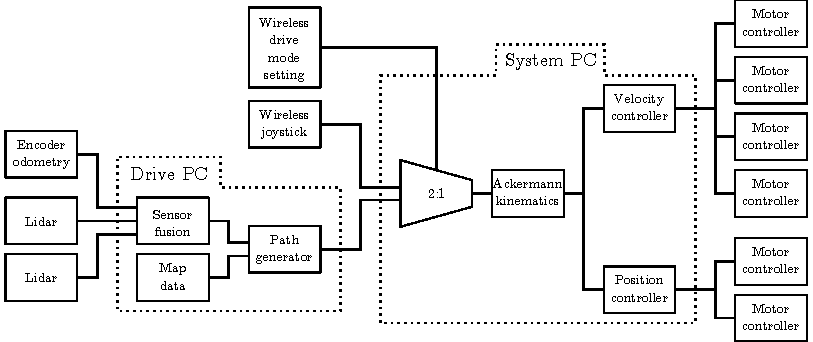
\includegraphics[width=\linewidth]{imgs/system_diagram/software.pdf}
        \caption{High level system diagram showing software architecture in terms of the manual and autonomous drive system.}
        \label{fig:system_diagram_software}
    \end{figure}

    A computer dedicated to processing sensing data related to navigation is connected to the platform's ``System PC'' via Ethernet.
    The open source Robotic Operating System (ROS) is used to facilitate communicate between the two computers.
    Not only is ROS used for inter-computer communication, but also within separate software nodes running on the same machine.
    Figure \ref{fig:system_diagram_software} shows the flow of data from various sources to the motor controllers.
    For simplicity it omits interface nodes, those used solely to interface the device to the ROS network.

    To maximise code reusablility, each device on the platform has its own node dedicated to publishing device data or subscribing to generated device commands.
    Examples of such devices are CAN adapters, motor controllers, wireless controllers, lidar, encoders.
    Nodes are also used to transform or perform calculations on available data as well as pass it between nodes written in either C++ or Python.

    In addition to the drive commands generated by the ``Drive PC'', a safety rated wireless controller lets the operator generate commands by joystick.
    The controller also has a mode selector that selects which commands are fed through to the motor drivers.
    An emergency stop button on the controller means that the platform can be stopped at any time.


\section{Autonomous Driving}
\label{sect:autonomous}
    \begin{figure}[htb]
        \centering
        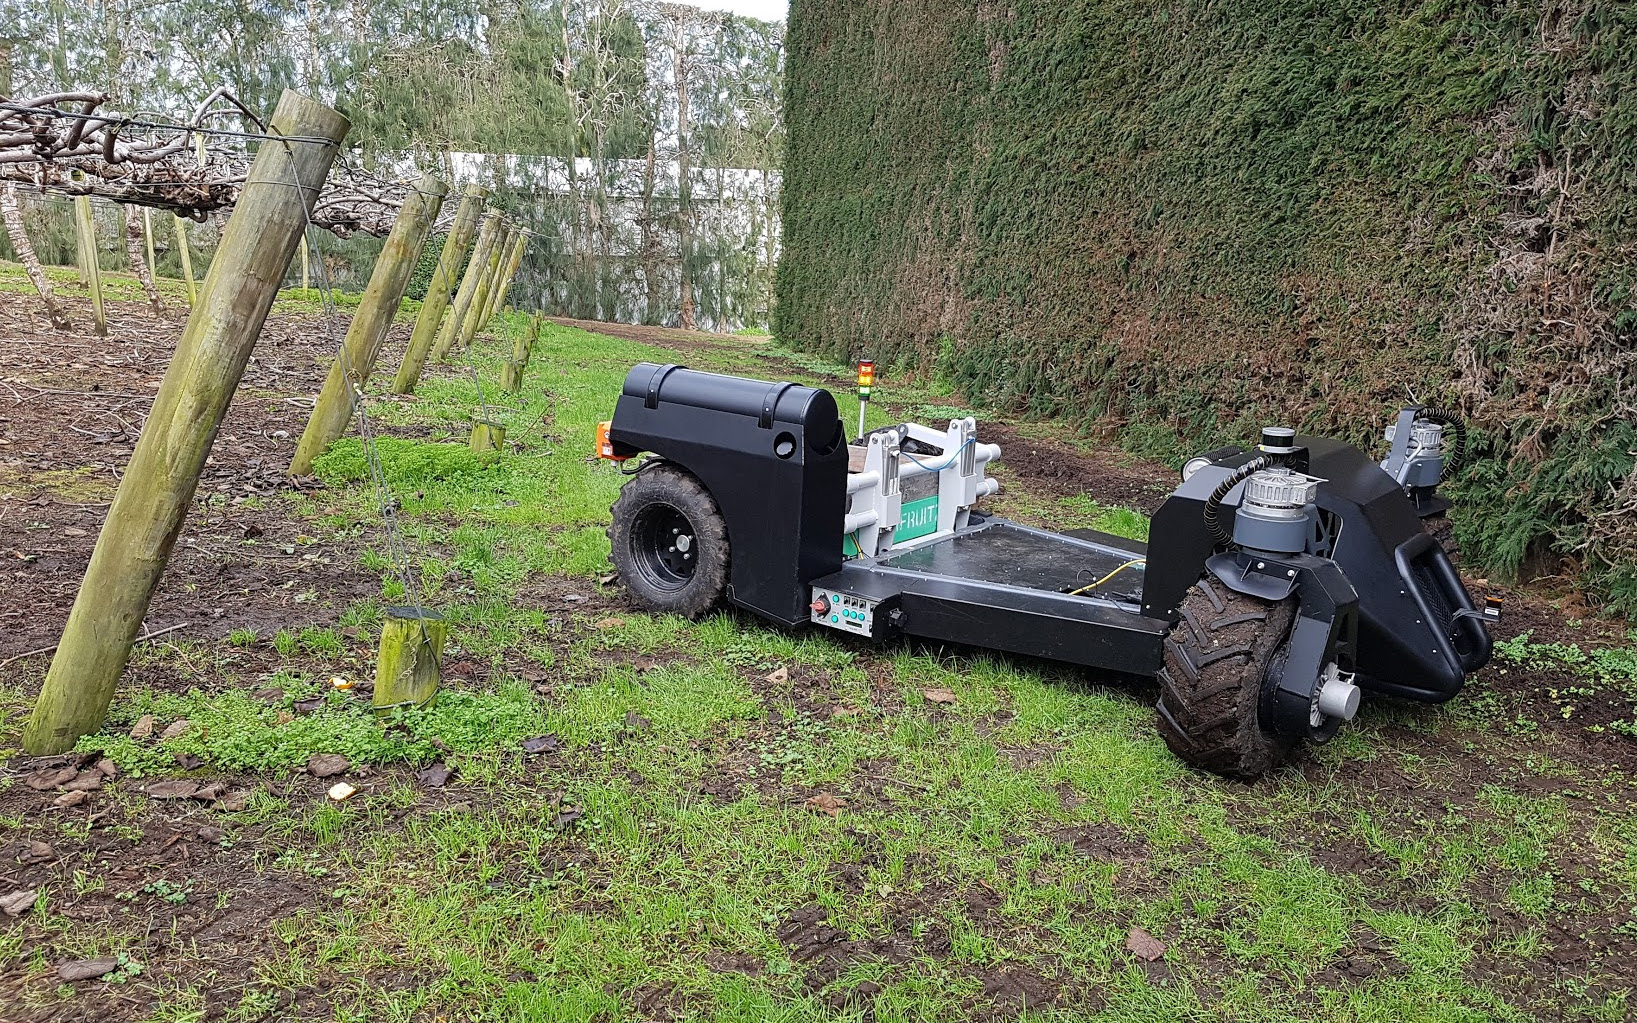
\includegraphics[width=\linewidth]{imgs/photos/suzy_turning.jpg}
        \caption{
            Photo showing the platform performing a row-end turn
        }
        \label{fig:suzy_turning}
    \end{figure}
    \color{red}
    Need content here.
    \color{black}
    Figure \ref{fig:suzy_turning} shows the AMMP turning, which is great.


\section{Discussion}
    TODO: Generally summerise the platform, its ability to carry stuff, suitability for the orchard environment, and its ability to drive autonomously.

\section*{Acknowledgements}
This research was funded in-part by a grant from the New Zealand Ministry of Business Innovation and Employment.
The authors acknowledge contributions from Phillip Ross, Gordon Neshausen, Josh Barnett and Erin Simms in the design and fabrication of the platform.

\section{Jamie-Mark communication}
You are free to suggest anything about anything.
Maybe you want to add someone to the authors list?
Maybe you don't like the focus of the review, or think a review is not necessary.
Perhaps you can think of something that would go well in the paper that I've not mentioned.

% Diagram of sensor placement
% Lidar units and visibility
% All electric drive system based on ackermann steering
% Sevcons modified to allow for direct CAN control.
% Power system and battery pack
% power-gen capable of charging battery pack approx 24hour duty
% Drive motors used as steering motors
% Control based on ROS, complete with gazebo simulation
% State the turning circle.
% State the mass and payload capability
% Show the area for drop-on modules (diagram)
% Integrated bin lifting mechanism
% Platform electronics

% Sections:
%   Mechanical design
%   Hardware and sensors
%   Software architecture


%% The Appendices part is started with the command \appendix;
%% appendix sections are then done as normal sections
%% \appendix

%% \section{}
%% \label{}

%% References
%%
%% Following citation commands can be used in the body text:
%%
%%  \citet{key}  ==>>  Jones et al. (1990)
%%  \citep{key}  ==>>  (Jones et al., 1990)
%%
%% Multiple citations as normal:
%% \citep{key1,key2}         ==>> (Jones et al., 1990; Smith, 1989)
%%                            or  (Jones et al., 1990, 1991)
%%                            or  (Jones et al., 1990a,b)
%% \cite{key} is the equivalent of \citet{key} in author-year mode
%%
%% Full author lists may be forced with \citet* or \citep*, e.g.
%%   \citep*{key}            ==>> (Jones, Baker, and Williams, 1990)
%%
%% Optional notes as:
%%   \citep[chap. 2]{key}    ==>> (Jones et al., 1990, chap. 2)
%%   \citep[e.g.,][]{key}    ==>> (e.g., Jones et al., 1990)
%%   \citep[see][pg. 34]{key}==>> (see Jones et al., 1990, pg. 34)
%%  (Note: in standard LaTeX, only one note is allowed, after the ref.
%%   Here, one note is like the standard, two make pre- and post-notes.)
%%
%%   \citealt{key}          ==>> Jones et al. 1990
%%   \citealt*{key}         ==>> Jones, Baker, and Williams 1990
%%   \citealp{key}          ==>> Jones et al., 1990
%%   \citealp*{key}         ==>> Jones, Baker, and Williams, 1990
%%
%% Additional citation possibilities
%%   \citeauthor{key}       ==>> Jones et al.
%%   \citeauthor*{key}      ==>> Jones, Baker, and Williams
%%   \citeyear{key}         ==>> 1990
%%   \citeyearpar{key}      ==>> (1990)
%%   \citetext{priv. comm.} ==>> (priv. comm.)
%%   \citenum{key}          ==>> 11 [non-superscripted]
%% Note: full author lists depends on whether the bib style supports them;
%%       if not, the abbreviated list is printed even when full requested.
%%
%% For names like della Robbia at the start of a sentence, use
%%   \Citet{dRob98}         ==>> Della Robbia (1998)
%%   \Citep{dRob98}         ==>> (Della Robbia, 1998)
%%   \Citeauthor{dRob98}    ==>> Della Robbia


%% References with bibTeX database:

\bibliographystyle{model5-names}
\bibliography{bibliography_jamie,bibliography_mark}


%% Authors are advised to submit their bibtex database files. They are
%% requested to list a bibtex style file in the manuscript if they do
%% not want to use model5-names.bst.

%% References without bibTeX database:

% \begin{thebibliography}{00}

%% \bibitem must have one of the following forms:
%%   \bibitem[Jones et al.(1990)]{key}...
%%   \bibitem[Jones et al.(1990)Jones, Baker, and Williams]{key}...
%%   \bibitem[Jones et al., 1990]{key}...
%%   \bibitem[\protect\citeauthoryear{Jones, Baker, and Williams}{Jones
%%       et al.}{1990}]{key}...
%%   \bibitem[\protect\citeauthoryear{Jones et al.}{1990}]{key}...
%%   \bibitem[\protect\astroncite{Jones et al.}{1990}]{key}...
%%   \bibitem[\protect\citename{Jones et al., }1990]{key}...
%%   \harvarditem[Jones et al.]{Jones, Baker, and Williams}{1990}{key}...
%%

% \bibitem[ ()]{}

% \end{thebibliography}

\end{document}

%%
%% End of file `elsarticle-template-5-harv.tex'.
